\documentclass[12pt]{article}

\usepackage[spanish, es-tabla, es-nodecimaldot]{babel}
\usepackage[utf8x]{inputenc}
\usepackage{amsmath}

\usepackage{hyperref}
\usepackage{url}
\usepackage{gensymb}
\usepackage[dvipsnames]{xcolor}

\usepackage{parskip}
\usepackage{fancyhdr}
\usepackage{multicol}
\usepackage{vmargin}
\usepackage{setspace}
\usepackage{geometry}

\usepackage{float}
\usepackage{array}
\usepackage{graphicx}
\graphicspath{{images/}}
\usepackage{wrapfig}
\usepackage{caption}
\usepackage{subcaption}

\setmarginsrb{2 cm}{1 cm}{2 cm}{1.5 cm}{1 cm}{1 cm}{1 cm}{1 cm}

\title{Equivalente Mecánico del Calor.}
\author{Martín Alejandro Paredes Sosa}		

\makeatletter
\let\thetitle\@title
\let\theauthor\@author
\let\thedate\@date										
\makeatother

\pagestyle{fancy}
\fancyhf{}
%\rhead{Lic.. Física}
%\lhead{Informe 5: \thetitle}
\cfoot{\thepage}

\begin{document}
%===================================================================================================
%====================================Titulo y Nombre================================================
%===================================================================================================
\begin{center}
{ \large \bfseries \thetitle}\\
\end{center}
	\begin{minipage}{\textwidth}
		\begin{center} 
			\theauthor 
			\end{center}
	\end{minipage}\\[-0.52 cm]
%===================================================================================================
\begin{abstract}
	En esta experiencia de laboratorio, se utilizo el ``\textit{Tubo de equivalente mecánico del calor}'', el cual tiene un sensor de temperatura, con el cual se midió el cambio de la temperatura en la placa de aluminio. Para tener el cambio en la temperatura, se giró el tubo con balines de acero, repetidamente, para que estos impactaran la placa. El objetivo de esto es obtener un valor numérico del equivalente mecánico del calor.

\end{abstract}
\vspace{-1cm}
%===================================================================================================
\section{Introducción}
\vspace{-0.5cm}
Esta experiencia en el laboratorio consistió en utilizar el ``\textit{Tubo de equivalente mecánico del calor}''. Este aparato nos permite medir la temperatura de una placa de aluminio. Cuando se le deja caer balines de acero repetidamente, la placa aumenta su temperatura levemente. El objetivo de este experimento, es demostrar los cambios en la energía gravitacional a la energía térmica y así tener un valor numérico del equivalente mecánico del calor. 

\hspace{0.5cm} Históricamente, tomo mucho tiempo en entender cuál era la naturaleza del calor. En un principio se pensó que este era un fluido, denominado calórico, que impregnaba los cuerpos y era responsable del calor que estos intercambiaban al estar en contacto. Para el siglo XIX, Joule ideó un experimento, donde demostraba que el calor era una forma de energía y que se podía obtener a partir de la energía mecánica. Joule se propuso demostrar que se podía elevar la temperatura del agua transfiriéndole energía mecánica. Este experimento se le conoce como ``experimento de Joule'' en el cual se determino el equivalente mecánico del calor.

\hspace{0.5cm}Antes del experimento, se pensaba que calor y energía eran dos magnitudes diferentes, por lo que las unidades en las que se median eran distintas. El calor se medía en con la caloría y la energía en joules. Una caloría se define como la cantidad de calor necesaria para elevar la temperatura de un gramo de agua destilada desde 14.5ºC a 15.5ºC. El descubrimiento de Joule llevó a la teoría de la conservación de la energía lo que a su vez condujo al desarrollo del primer principio de la Termodinámica.\vspace{-0.5cm}
%===================================================================================================
\section{Desarrollo Experimental}\vspace{-0.5cm}
Primeramente, se investigaron las capacidades calorificas del aluminio y del acero, ya que la placa es de aluminio y los balines de acero. Para empezar con el experimento se midió la masa de la placa y luego la de los 60 balines. Luego se midieron las dimensiones del tubo.

\begin{figure}[H]
\centering
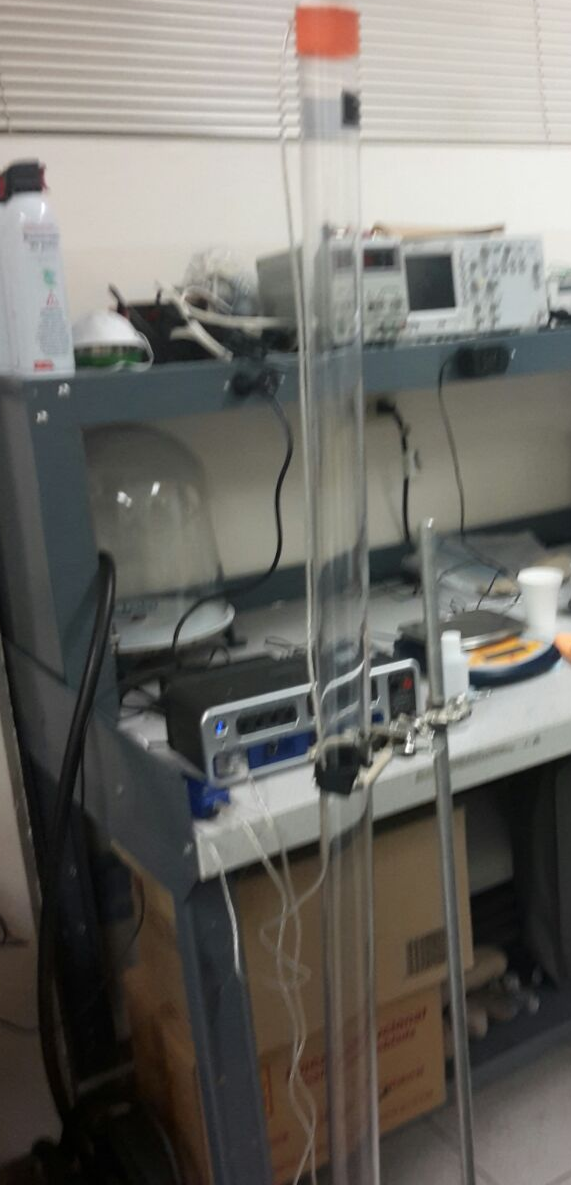
\includegraphics[width=0.25\linewidth ,height=5cm]{Arreglo.png}
\caption{Arreglo Experimental}
\label{fig:Arreglo}
\end{figure}

Se colocó el tubo en la base mostrada en la figura \ref{fig:Arreglo}. Se conecto el termistor de respuesta rápida de la placa a la interfaz.  En DataStudio se configuro un experimento que utilizara el termistor con una frecuencia de muestreo de 20 Hz y 100 Hz. Se colocaron 60 balines dentro del tubo y se tapo. Se inició la toma de datos y se procedió a girar el tubo repetidamente. Se giro aproximadamente 4 veces por medición. 

Se volvió a realizar el experimento, pero ahora se varió la cantidad de balines en el tubo. Primero  con 80 balines, luego se realizo con 100 y 120 balines con las mismas frecuencia de muestreo.

%===================================================================================================
\section{Resultados}
La tabla \ref{tab:Med} muestra las mediciones que se realizaron antes de empezar el experimento.

	\begin{table}[H]
		\centering
		\begin{tabular}{|c|c|}
			\hline
			\textbf{Medición} & \textbf{Valor} \\ \hline
			 Masa Placa & 1.5672$\pm$0.00003 g \\ \hline
			 Masa de 60 balines & 20.5653$\pm$0.00003 g \\ \hline
			 Masa de 80 balines & 27.4730$\pm$0.00003 g \\ \hline
			 Masa de 100 balines & 34.3130$\pm$0.00003 g \\ \hline
			 Masa de 120 balines & 41.1839$\pm$0.00003 g \\ \hline
			 Longitud del Tubo & 90.6 $\pm$0.47cm  \\ \hline
			 Temperatura Ambiente & 26.933$\pm$0.323°C \\ \hline
		\end{tabular}
		\caption{Mediciones del Aparato}
		\label{tab:Med}
	\end{table}
	
En la figura \ref{fig:med} se muestra manera de gráfica los resultados del experimento.

	\begin{figure}[H]
		\centering
		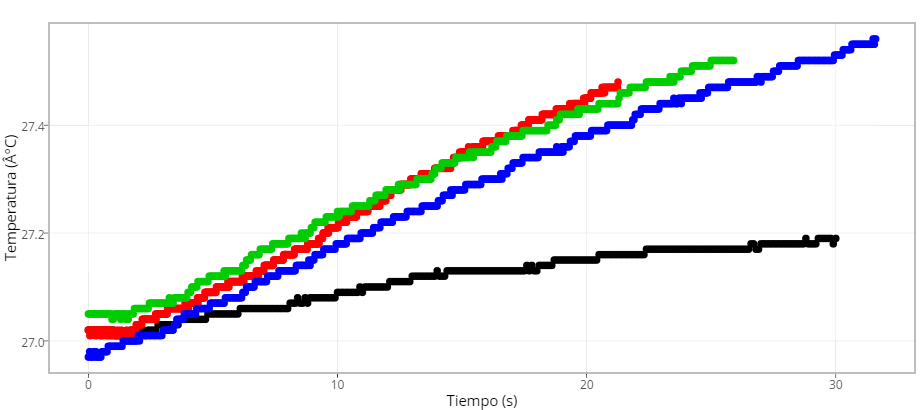
\includegraphics[width = 0.75\linewidth]{medi.png}
		\caption{Mediciones experimentales}
		\label{fig:med}
	\end{figure}

Para obtener un equivalente es necesario obtener la energía potencial y la energía en forma de calor del proceso de girar el tubo. La energía potencial gravitacional esta dada por 
\begin{equation}
\label{eq:poten}
E_p = m_bgh
\end{equation}
donde $m_b$ es la masa de los balines que caen, $g$ es la aceleración de la gravedad y $h$ es la distancia recorrida (dos veces la longitud del tubo). Como se vario la masa (cantidad de balines), la energía potencial cambia según sea la cantidad de balines que estén en el tubo. La tabla \ref{tab:PE} muestra la energía potencial para cada caso.
	
	\begin{table}[H]
		\centering
		\begin{tabular}{|c|c|}
			\hline
			\textbf{Numero de Balines} & \textbf{Energía Potencial} ($E_p$) \\ \hline
			60   & 0.3656  J \\ \hline
			80   & 0.4884  J \\ \hline
			100  & 0.6099  J \\ \hline
			120  & 0.7321  J \\ \hline
		\end{tabular}
		\caption{Energía Potencial por la cantidad de balines en un giro.}
		\label{tab:PE}
	\end{table}
	
Para encontrar el calor (Q) se hace uso de la siguiente expresión:
\begin{equation}\label{eq:Q}
Q = (m_p c_p + m_b c_b) \Delta T
\end{equation}
donde $m_p$ es la masa de la placa, $c_p = 0.215 \frac{cal}{g°C}$ el calor especifico del calor especificó de la placa y $c_b = 0.114 \frac{cal}{g°C}$  el de los balines.

El experimento se realizó variando la cantidad de balines. El la tabla \ref{tab:Q60} se muestra el calor calculado utilizando la ecuación \eqref{eq:Q} para cada cantidad de balines.
	
	\begin{table}[H]
		\centering
		\begin{tabular}{|c|c|c|}
			\hline
			\textbf{Balines} & $\Delta$ \textbf{T} & \textbf{Calor} (Q) \\ \hline
			60   & 0.16°C  & 0.4322 cal \\ \hline
			80   & 0.36°C  & 1.2586 cal \\ \hline
			100  & 0.39°C  & 1.6702 cal \\ \hline
			120  & 0.59°C  & 2.9929 cal \\ \hline
		\end{tabular}
		\caption{Calor obtenido.}
		\label{tab:Q60}
	\end{table}

La tabla \ref{tab:Comp} nos muestra la relación entre la energía potencial gravitacional y la energía en forma de calor.
	
	\begin{table}[H]
		\centering
		\begin{tabular}{|c|c|c|c|}
			\hline
			Balines & $E_p$ & Q & $E_p$/Q\\ \hline
			60  & 1.8280  J & 0.4322 cal & 4.2295 J/cal \\ \hline
			80  & 6.3492  J & 1.2586 cal & 5.0447 J/cal \\ \hline
			100 & 9.1485  J & 1.6702 cal & 5.4775 J/cal  \\ \hline
			120 & 12.4457 J & 2.9929 cal & 4.1584 J/cal \\ \hline
			\multicolumn{3}{|c|}{\textbf{Promedio}} & 4.7275 J/cal \\ \hline
		\end{tabular}
		\caption{Energía Potencial transformada en calor.}
		\label{tab:Comp}
	\end{table}
\pagebreak
%===================================================================================================
\section{Discusión} 
Se llego a que la equivalencia entre unidades de calor y energía es 4.7275 J/cal mientras los textos nos dicen que dicho valor es de 4.18 J/cal. Por lo tanto, el experimento nos da una buena aproximación del equivalente mecánico del calor, de hecho se tiene un 13.1\% de error. Este valor se ha calculado con diversos experimentos, y con este experimento se obtuvo un buen resultado.

%===================================================================================================
\section{Conclusiones}
Se llegó a que existe una relación entre la energía mecánica y el calor, ya que se observó un aumento en la temperatura cuando los balines colisionaban con la placa. El procedimiento que se siguió, fue adecuado, ya que nos llevo a un resultado cercano al encontrado en los textos y tablas. 
%================================================================================================


\begin{thebibliography}{3}
	\bibitem{acu}
		Acuña, H. (2015). \textit{Manual de Guías de Experiencias en el Laboratorio de Termodinámica Clásica}.

	\bibitem{Joule}
		Serrano Fernandez, A., Martín Blas, T. (s.f.) \emph{Equivalente mecánico del calor} Recuperado el 14 de Mayo de 2017 de \url{http://acer.forestales.upm.es/basicas/udfisica/asignaturas/fisica/termo1p/joule.html}
	
	\bibitem{Pasco}
		Pasco (s.f.) \textit{Mechanical Equivalent of Heat Tube} Recuperado el 14 de Mayo de 2017 de \url{www.pasco.com}
\end{thebibliography}
%================================================================================================

\end{document}

